\documentclass[12pt,a4paper,notitlepage]{article}
% dans ce modèle article ne pas utiliser la mention "chapter", par contre on peut
% utiliser la numérotation naturelle et les références croisées.
\usepackage[utf8x]{inputenc}
\usepackage{ucs}
\usepackage[french]{babel}
\usepackage[T1]{fontenc}
%\usepackage{eurosym} % pour pouvoir utiliser le symbole \euro{}
\usepackage[left=17mm,right=17mm,top=17mm,bottom=17mm]{geometry}
% définition du nombre de lignes à afficher en fin ou en début de page pour
% éviter les veuves et orphelines.
\usepackage[all, defaultlines=3]{nowidow}
\usepackage{array}
\usepackage[table]{xcolor} % pour couleur de blocs, permis avec \color{couleur}{texte}

\usepackage{multirow}
\usepackage{multicol}
	\setlength{\columnsep}{0.6cm}
	\setlength{\columnseprule}{1pt}
	\def\columnseprulecolor{\color{black}}

%\usepackage{wrapfig}
% \begin{wrapfigure}[lineheight]{position = r R l L i I o O}{width}
%  minuscule = float, majuscule = force emplacement
% \end{wrapfigure}

\usepackage{hyperref} %support des url via le tag \url
\hypersetup{
	colorlinks=true,
	linkcolor=blue,
	urlcolor=purple,
	}
	\urlstyle{same}
\usepackage{amsmath}
\usepackage{amsfonts}
\usepackage{amssymb}

\usepackage{textcomp}

\usepackage{graphicx}
%\graphicspath{ {./Images/} } % indique le chemin relatif où sont situées les images
% définition de la clé Graphic Inclusion pour paramétrer par défaut la taille des images incluses
	\setkeys{Gin}{width=0.7071\linewidth}
\usepackage{float}
	\floatplacement{table}{H} %par défaut tables là où code est posé
	\floatplacement{figure}{H} %par défaut images là où code est posé
\usepackage{siunitx}
	\sisetup{locale = FR}
%%%% Packet circuitikz permet de dessiner des circuits électriques, peut nécessiter l'utiliation de siunitx
%\usepackage[european]{circuitikz}
%\usetikzlibrary{babel}
%\usepackage{qrcode}
%\usepackage{pgfplots} %permet de tracer directement des graphiques depuis latex

\usepackage{ifthen}
%%% Gestion de la dyslexie
\newboolean{isDyslexique}
	\setboolean{isDyslexique}{false}
%%% Gestion de la correction
\newboolean{isCorrection}
	\setboolean{isCorrection}{false}

% \usepackage{palatino} %\usepackage{sans}
% \usepackage{lxfonts} %\usepackage{arev}
\ifthenelse{\boolean{isDyslexique}}{% si vrai :
	\usepackage{arev}
	\renewcommand{\baselinestretch}{1.5}
}{% si faux :
	\usepackage{lmodern}
	\renewcommand{\baselinestretch}{1.25}
}
\usepackage{lastpage}
% test de modification des headers et footers
\usepackage{fancyhdr}
\pagestyle{fancy}
\fancyhf{}
\fancyhead[LE,RO]{\rightmark}
\fancyhead[LO,RE]{\leftmark}
\fancyfoot[LE,RO]{F.S.G.}
\fancyfoot[C]{.::--- \ \thepage / \pageref*{LastPage} \ ---::.}
\fancyfoot[RE,LO]{Titre}
% fin du test de modification :)
\usepackage{tikz}
	\usetikzlibrary{babel,math}
% inclusion du paquet bclogo pour boîtes avec logo de mise en exergue
\usepackage[tikz]{bclogo}

% ========= DÉFINITION D'UN INTERLIGNE DIFFÉRENT ===============
\setlength{\parskip}{0.1cm} % définit l'espacement entre paragraphes
\renewcommand{\thesection}{\Roman{section}}

\author{F.G.}
% éviter le titre peut-être ?
\title{}

\begin{document}

\begin{flushleft}
\begin{tabular}{| m{0.15\linewidth}  m{0.8\linewidth} || }
	\hline
	\multirow{4}{*}{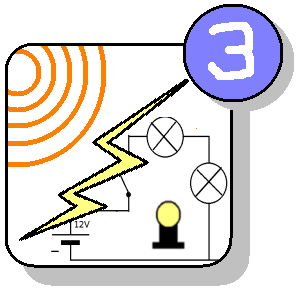
\includegraphics[width=\linewidth]{cycle3-logo-elec-ondes-nrj.png}} 
	& cx-x·p·ac
	\begin{LARGE}
		Ici il faut écrire le titre de l'activité qui va bien !!!
	\end{LARGE} \cr
	\cline{2-2}
	 & \cr
	 & Nom : . \ \ . \ \ . \ \ . \ \ . \ \ . \ \ . \ \ . Prénom : . \ \ . \ \ . \ \ . \ \ . \ \ . \cr
	 & \cr
	 & Classe / Groupe : . \ \ . \ \ . \ \ . Durée : ..... min. \cr
	\hline\hline
\end{tabular}
\end{flushleft}

% ======== LISTE DES IMAGES DISPONIBLES POUR CYCLES 3 ET 4 =========
% 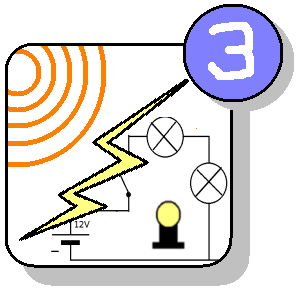
\includegraphics[scale=0.333]{cycle3-logo-elec-ondes-nrj.png}
% 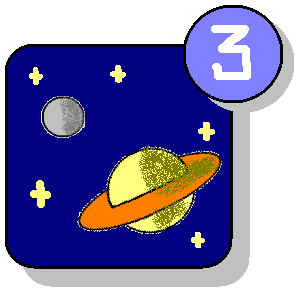
\includegraphics[scale=0.333]{cycle3-logo-espace.png}
% 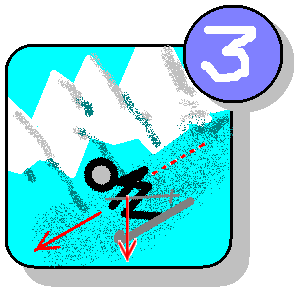
\includegraphics[scale=0.333]{cycle3-logo-mvts.png}
% 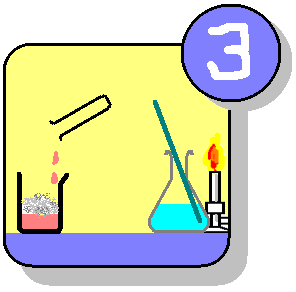
\includegraphics[scale=0.333]{cycle3-logo-transfo-matiere.png}
% 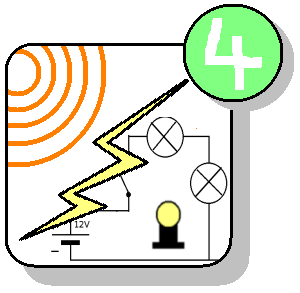
\includegraphics[scale=0.333]{cycle4-logo-elec-ondes-nrj.png}
% 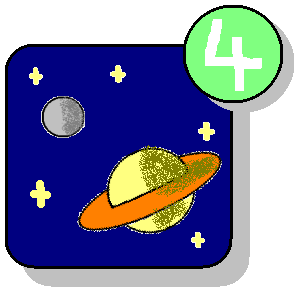
\includegraphics[scale=0.333]{cycle4-logo-espace.png}
% 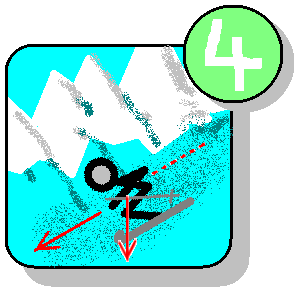
\includegraphics[scale=0.333]{cycle4-logo-mvts.png}
% 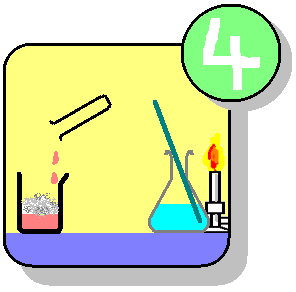
\includegraphics[scale=0.333]{cycle4-logo-transfo-matiere.png}

\begin{flushleft}
\begin{tabular}{| m{0.15\linewidth} | m{0.8\linewidth} ||}
	\hline
	NOTE : & APPRÉCIATION : \cr
	$ ~~ $ & $ ~~ $ \cr
	$ ~~ $ & $ ~~ $ \cr
	$ ~~ $ & $ ~~ $ \cr
	$ ~~ $ & $ ~~ $ \cr
	$ ~~ $ & $ ~~ $ \cr
	\hline\hline
\end{tabular}
\end{flushleft}

% $ ~~ $

\begin{flushleft}
\begin{tabular}{| m{0.03\linewidth} | m{0.75\linewidth} || m{0.015\linewidth} | m{0.015\linewidth} | m{0.015\linewidth} | m{0.015\linewidth} || }
\hline
\multirow{2}{*}{Ref} & \multirow{2}{*}{i~n~t~i~t~u~l~é~~~ d~e~~~ l~a~~~ c~o~m~p~é~t~e~n~c~e (cycle4) } & \multicolumn{4}{c ||}{É~t~a~t} \cr
	\cline{3-6}
	& & I & F & S & T \cr \hline
% A & Pratiquer des démarches scientifiques \cr \hline
	A1 & \footnotesize{Identifier des questions de nature scientifique.} & & & & \cr \hline
	A2 & \footnotesize{Proposer une ou des hypothèses pour répondre à une question scientifique. \newline Concevoir une expérience pour la ou les tester.} & & & & \cr \hline
	A3 & \footnotesize{Mesurer des grandeurs physiques de manière directe ou indirecte.} & & & & \cr \hline
	A4 & \footnotesize{Interpréter des résultats expérimentaux, en tirer des conclusions et les communiquer en argumentant.} & & & & \cr \hline
	A5 & \footnotesize{Développer des modèles simples pour expliquer des faits d'observations et mettre en \oe{}uvre des démarches propres aux sciences.} & & & & \cr \hline
% B & Concevoir, créer, réaliser \cr \hline
	B1 & \footnotesize{Concevoir et réaliser un dispositif de mesure ou d'observation.} & & & & \cr \hline
% C & S'approprier des outils et des méthodes \cr \hline
	C1 & \footnotesize{Effectuer des recherches bibliographiques.} & & & & \cr \hline
	C2 & \footnotesize{Utiliser des outils numériques pour mutualiser des informations sur un sujet scientifique.} & & & & \cr \hline
	C3 & \footnotesize{Planifier une tâche expérimentale, organiser son espace de travail, garder des traces des étapes suivies et des résultats obtenus.} & & & & \cr \hline
% D & Pratiquer des langages \cr \hline
	D1 & \footnotesize{Lire et comprendre des documents scientifiques.} & & & & \cr \hline
	D2 & \footnotesize{Utiliser la langue française en cultivant précision, richesse de vocabulaire et syntaxe pour rendre compte des observations, expériences, hypothèses et conclusions.} & & & & \cr \hline
	D3 & \footnotesize{S'exprimer à l'oral lors d'un débat scientifique.} & & & & \cr \hline
	D4 & \footnotesize{Passer d'une forme de langage scientifique à une autre.} & & & & \cr \hline
% E & Mobiliser des outils numériques \cr \hline
	E1 & \footnotesize{Utiliser des outils d'acquisition et de traitement de données, de simulations et de modèles numériques.} & & & & \cr \hline
	E2 & \scriptsize{Produire des documents scientifiques grâce à des outils numériques, en utilisant l'argumentation et le vocabulaire spécifique à la physique et à la chimie.} & & & & \cr \hline
% F & Adopter un comportement éthique et responsable \cr \hline
	F1 & \scriptsize{Expliquer les fondements des règles de sécurité en chimie, électricité et acoustique. Réinvestir ces connaissances ainsi que celles sur les ressources et sur l'énergie, pour agir de façon responsable.} & & & & \cr	\hline
	F2 & \footnotesize{S'impliquer dans un projet ayant une dimension citoyenne.} & & & & \cr	\hline
% G & Se situer dans l'espace et dans le temps \cr \hline
	G1 & \footnotesize{Expliquer, par l'histoire des sciences et des techniques, comment les sciences évoluent et influencent la société.} & & & & \cr	\hline
	G2 & \footnotesize{Identifier les différentes échelles de structuration de l'Univers.} & & & & \cr \hline
	\hline
\end{tabular}
\end{flushleft}

\begin{flushleft}
\begin{tabular}{| m{0.04\linewidth} | m{0.74\linewidth} || m{0.015\linewidth} | m{0.015\linewidth} | m{0.015\linewidth} | m{0.015\linewidth} || }
\hline
\multirow{2}{*}{Ref} & \multirow{2}{*}{i~n~t~i~t~u~l~é~~~ d~e~~~ l~a~~~ c~o~m~p~é~t~e~n~c~e (cycle3) } & \multicolumn{4}{m{0.05\linewidth} ||}{É~t~a~t} \cr
	\cline{3-6}
	& & I & F & S & T \cr \hline
% A. & Pratiquer des démarches scientifiques et technologiques & & & & \cr \hline
	A.1. & formuler une question ou une problématique scientifique ou technologique simple & & & & \cr \hline
	A.2. & proposer une ou des hypothèses pour répondre à une question ou un problème & & & & \cr \hline
	A.3. & proposer des expériences simples pour tester une hypothèse & & & & \cr \hline
	A.4. & interpréter un résultat, en tirer une conclusion & & & & \cr \hline
	A.5. & formaliser une partie de sa recherche sous une forme écrite ou orale & & & & \cr \hline
% B. & Concevoir, créer, réaliser & & & & \cr \hline
	B.1. & Identifier les évolutions des besoins et des objets techniques dans leur contexte. & & & & \cr \hline
	B.2. & Identifier les principales familles de matériaux & & & & \cr \hline
	B.3. & Décrire le fonctionnement d’objets techniques, leurs fonctions et leurs composants & & & & \cr \hline
	B.4. & Réaliser en équipe tout ou une partie d’un objet technique répondant à un besoin. & & & & \cr \hline
	B.5. & Repérer et comprendre la communication et la gestion de l’information. & & & \cr \hline
% C. & S’approprier des outils et des méthodes & & & & \cr \hline
	C.1. & Choisir ou utiliser le matériel adapté pour mener une observation, effectuer une mesure, réaliser
une expérience ou une production & & & & \cr \hline
	C.2. & Faire le lien entre la mesure réalisée, les unités et l’outil utilisés.. & & & & \cr \hline
	C.3. & Garder une trace écrite ou numérique des recherches, des observations et des expériences réalisées. & & & & \cr \hline
	C.4. & Organiser seul ou en groupe un espace de réalisation expérimentale. & & & & \cr \hline
	C.5. & Effectuer des recherches bibliographiques simples et ciblées. \newline Extraire les informations pertinentes
d’un document et les mettre en relation pour répondre à une question. & & & & \cr \hline
	C.6. & Utiliser les outils mathématiques adaptés. & & & & \cr \hline
% D. & Pratiquer des langages & & & & \cr \hline
	D.1. & Rendre compte des observations, expériences, hypothèses, conclusions en utilisant un vocabulaire
précis. & & & & \cr \hline
	D.2. & Exploiter un document constitué de divers supports (texte, schéma, graphique, tableau, algorithme
simple). & & & & \cr \hline
	D.3. & Utiliser différents modes de représentation formalisés (schéma, dessin, croquis, tableau, graphique,
texte). & & & & \cr \hline
	D.4. & Expliquer un phénomène à l’oral et à l’écrit. & & & & \cr \hline
% E. & Mobiliser des outils numériques & & & & \cr \hline
	E.1. & Utiliser des outils numériques pour communiquer des résultats & & & & \cr \hline
	E.2. & Utiliser des outils numériques pour traiter des données & & & & \cr \hline
	E.3. & Utiliser des outils numériques pour simuler des phénomènes & & & & \cr \hline
	E.4. & Utiliser des outils numériques pour représenter des objets techniques & & & & \cr \hline
	E.5. & Identifier des sources d’informations fiables. & & & & \cr \hline
% F. & Adopter un comportement éthique et responsable & & & & \cr \hline
	F.1. & Relier des connaissances acquises en sciences et technologie à des questions de santé, de sécurité et d’environnement. & & & & \cr \hline
	F.2. & Mettre en œuvre une action responsable et citoyenne, individuellement ou collectivement, en et hors milieu scolaire, et en témoigner. & & & & \cr \hline
% G. & Se situer dans l’espace et dans le temps & & & & \cr \hline
	G.1. & Replacer des évolutions scientifiques et technologiques dans un contexte historique, géographique, économique et culturel. & & & & \cr \hline
	G.2. & Se situer dans l’environnement et maitriser les notions d’échelle. & & & & \cr \hline
\hline % double ligne finale
\end{tabular}
\end{flushleft}
% ============= DÉBUT DU DOCUMENT DE TRAVAIL ==================


\end{document}

%%%%%%%%%%%%%%%%%%%%%%%%%%%%%%%%%%%%%%%%%%%%%%%%%%%%%%%

% cadre pour le cours / à savoir par coeur.
\begin{bclogo}[couleur=pink!5, epOmbre=0.2cm, arrondi=0.1, logo=\bccoeur, nobreak=true]{}

\end{bclogo}

% cadre pour un document à analyser (informatif)
\begin{bclogo}[couleur=blue!5, epOmbre=0.2cm, arrondi=0.1, logo=\bcinfo, nobreak=true]{}

\end{bclogo}

% cadre pour le travail :
\begin{bclogo}[couleur=yellow!5, arrondi=0.1, logo=\bccrayon, nobreak=true]{}

\end{bclogo}
